\section{Estado del Arte}

\begin{frame}{Redes neuronales}

	\centering
 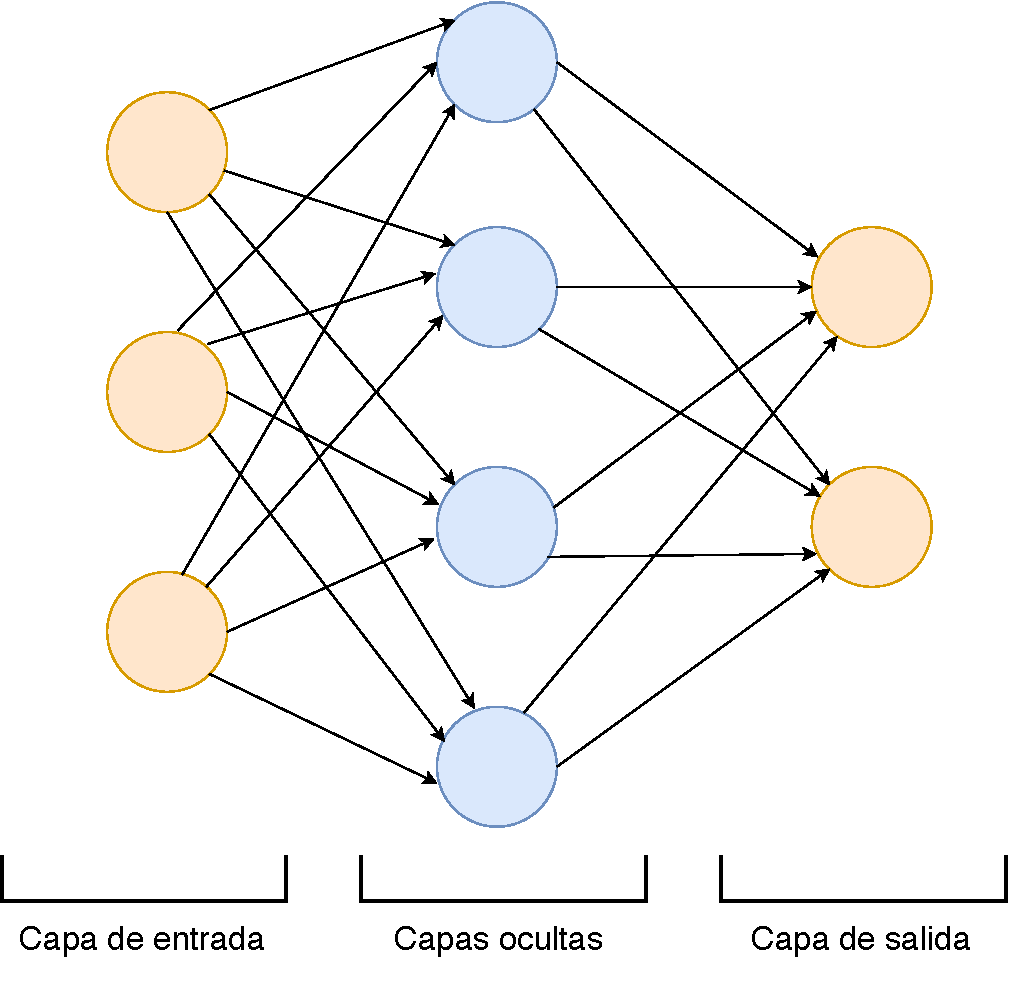
\includegraphics[width=0.5\textwidth]{fig/redneuronal.pdf}

\end{frame}

\begin{frame}{Redes neuronales}
\framesubtitle{FCN AlexNet}

	\centering
 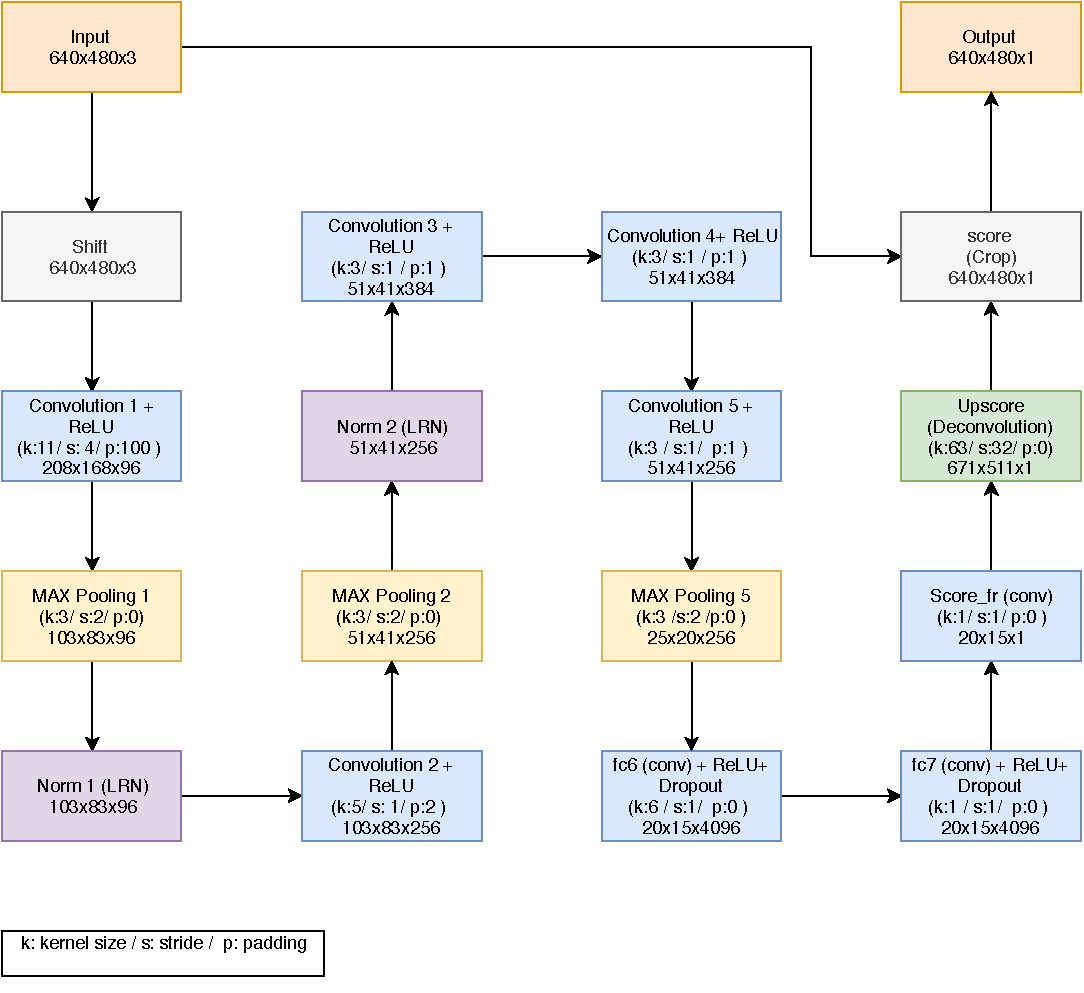
\includegraphics[width=0.7\textwidth]{anexo/FCN-Alex.pdf}
\end{frame}

\begin{frame}{Redes neuronales}
\framesubtitle{Simple Feature Extraction}
	\centering
 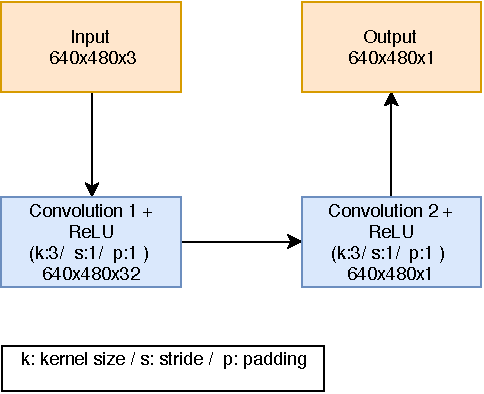
\includegraphics[width=0.4\textwidth]{anexo/sfe.pdf}
\end{frame}

\begin{frame}{Redes neuronales}
\framesubtitle{SFEwAN}
	\centering
 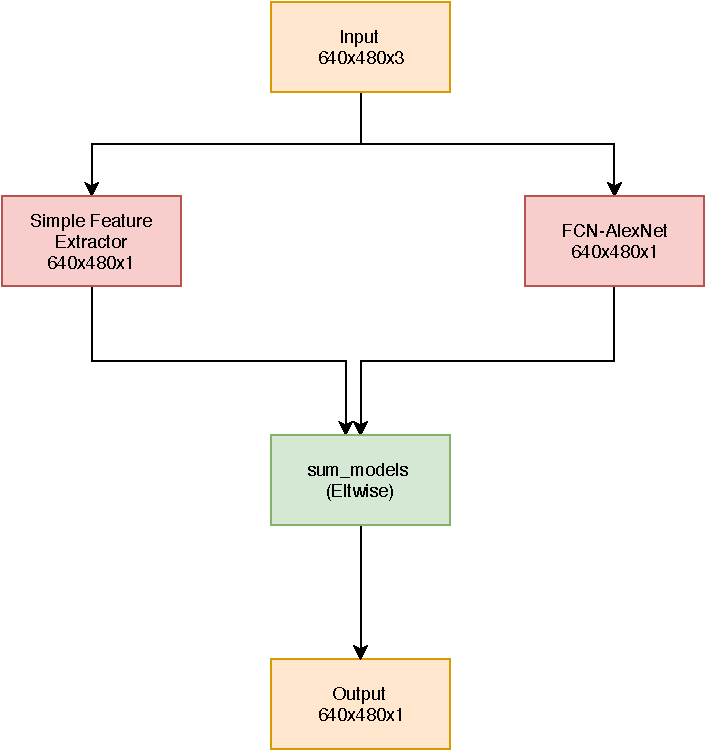
\includegraphics[width=0.6\textwidth]{anexo/sfewan.pdf}
\end{frame}




\begin{frame}{Herramientas de desarrollo para redes neuronales}

	\centering
 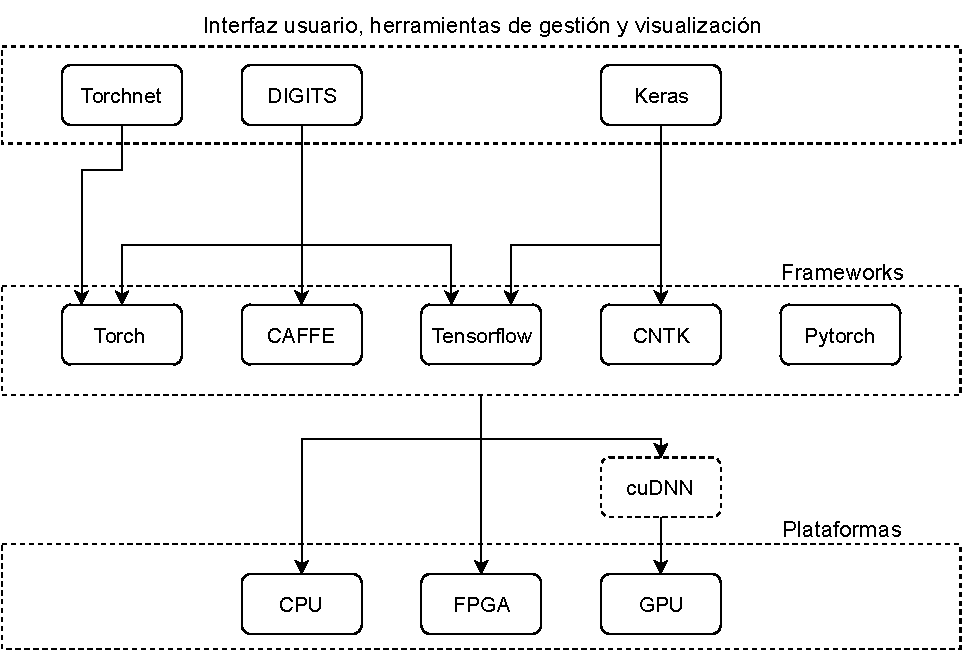
\includegraphics[width=0.9\textwidth]{fig/DL-frameworks.pdf}

\end{frame}


\begin{frame}{Programación paralela}

\centering
 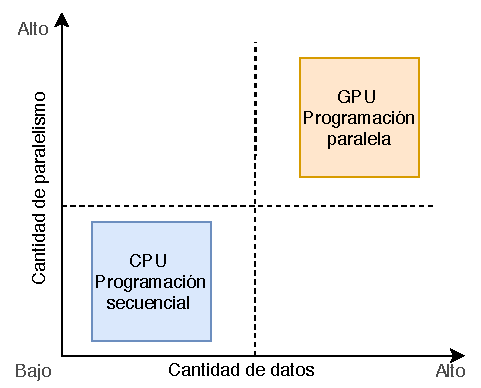
\includegraphics[width=0.6\textwidth]{fig/paralelismo.pdf}

\end{frame}


\begin{frame}{Sistemas basados en GPU}
\resizebox{\linewidth}{!}{% Resize table to fit within \linewidth horizontally
\begin{table}[]
\centering
\begin{tabular}{lccccc}
\toprule
             & Jetson TX2                                                          & Jetson AGX Xavier & Laptop 950M                                                   & Sistema 1080Ti                                                 & Sistema TITAN RTX                                              \\ \midrule
CUDA cores   & 256                                                                 & 512               & 640                                                           & 3584                                                           & 4608                                                           \\
Tensor cores & -                                                                   & 64                & -                                                             & -                                                              & 576                                                            \\
CC           & 6.2                                                                 & 7.2               & 5.0                                                             & 6.0                                                              & 7.5                                                            \\
CPU          & \begin{tabular}[c]{@{}c@{}}Denver 2-core \\ ARM 4-core\end{tabular} & ARM 8-core        & \begin{tabular}[c]{@{}c@{}}Intel core \\ i7-6700\end{tabular} & \begin{tabular}[c]{@{}c@{}}Intel core\\  i5-8600K\end{tabular} & \begin{tabular}[c]{@{}c@{}}Intel core \\ i5-8600K\end{tabular}\\
\bottomrule
\end{tabular}
\end{table}
}
\centering
 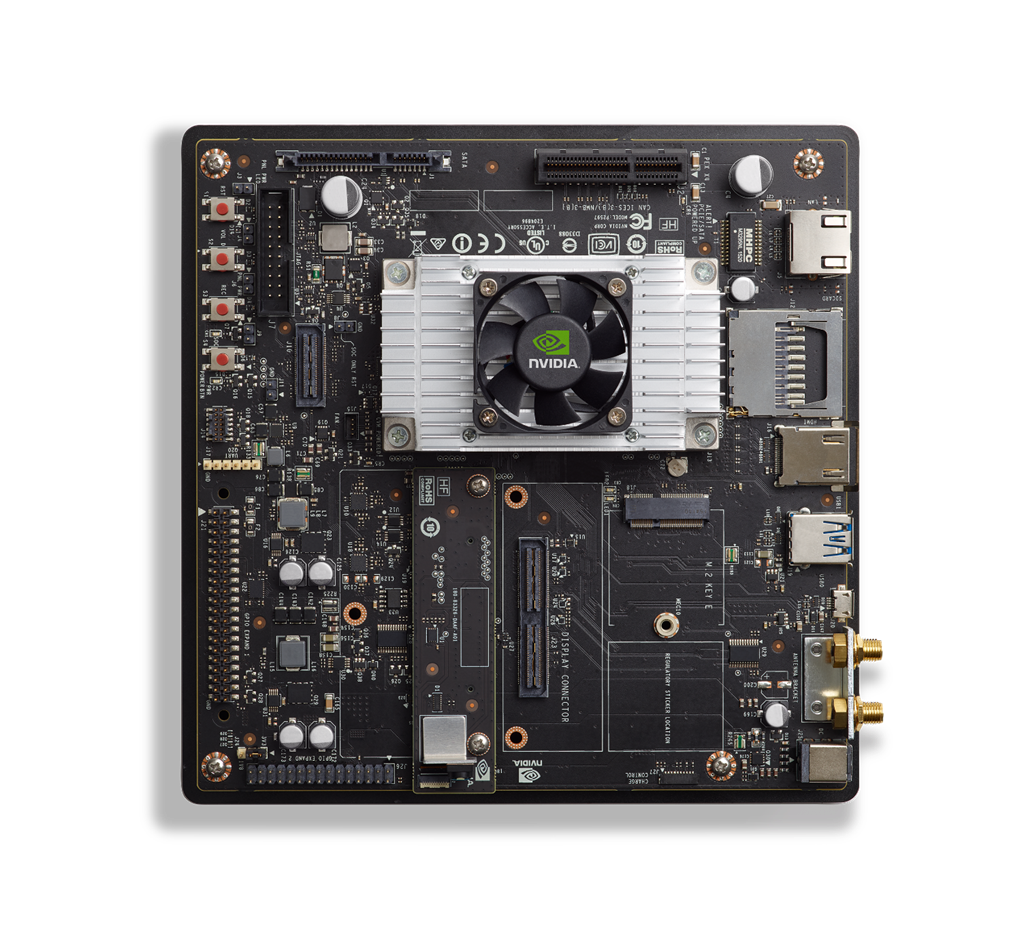
\includegraphics[width=0.3\textwidth]{fig/JTX2.png}
  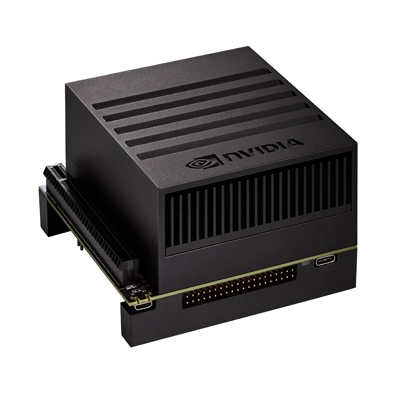
\includegraphics[width=0.25\textwidth]{fig/XAVIER.jpg}
    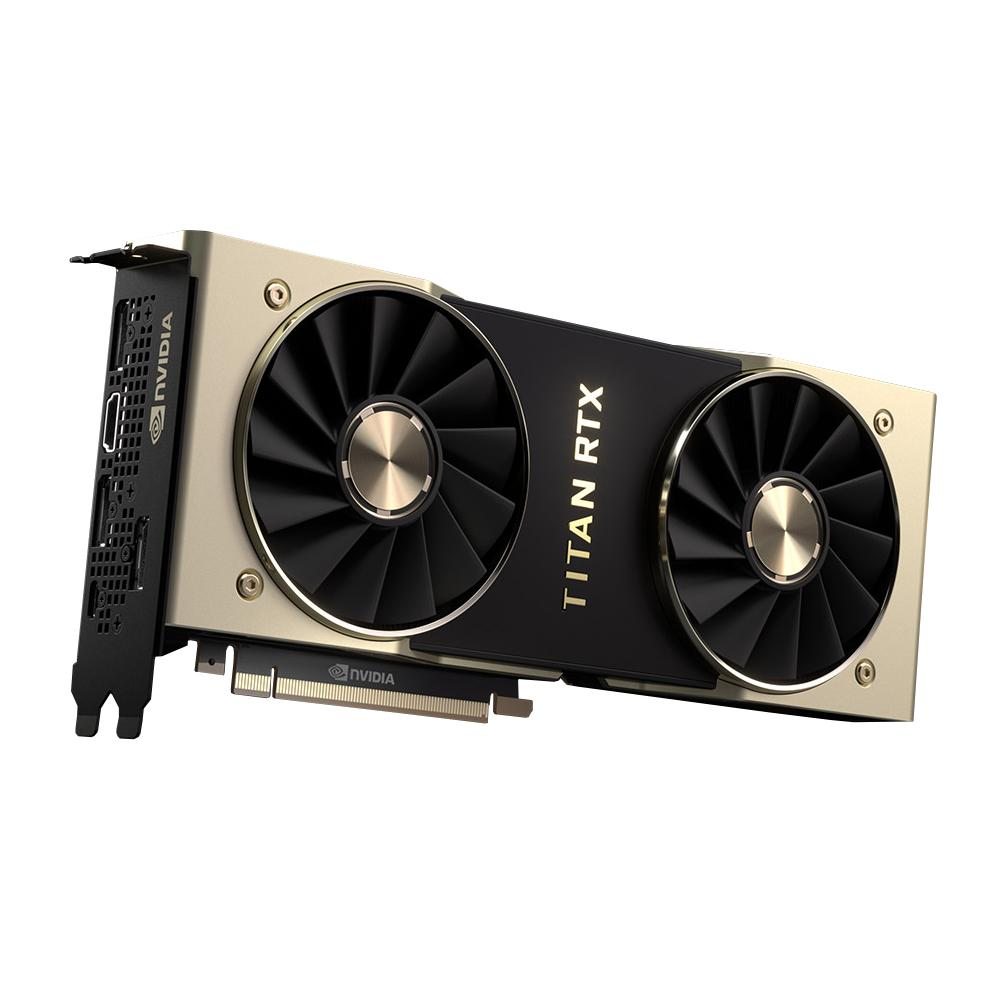
\includegraphics[width=0.3\textwidth]{fig/titan.jpg}
  \end{frame}


